\chapter{Roadmap Methods for Motion Planning}
\label{chap:roadmaps}

Robots are fundamentally agents that move through the world,
and so the question of how to best deliberate about motion
is a central problem in robotics.
Different tasks and problem domains expose a vast array of
qualities and properties of motion that are important
-- for example, motion that is expressive, efficient, or expected
-- and algorithms can rely on a rich and growing set
of models and methodologies in order to generate such motion.

Underlying this rich tapestry of robotic motion
is the most fundamental abstraction of motion planning --
finding a path for a system which accomplishes a motion task
without colliding with obstacles.
While this might at first seem straightforward,
finding such paths for articulated robotics in
complex semi-structured environments
is no easy feat,
and finding such paths quickly and efficiently
is of utmost importance.

This chapter includes a brief introduction to
the motion planning problem.
Due to its paramount importance to robotics,
variations on this problem have deservedly
enjoyed a considerable amount of attention over the past 40 years.
We tailor our investigation towards aspects of the problem
that are relevant to this thesis
-- for a comprehensive treatment,
we refer to LaValle \citep{lavalle2006planningbook}
and Choset et. al. \citep{choset2005robotmotion}.
In particular,
we provide an overview of a class of approaches called roadmap methods
that are well-suited to motion planning for articulated robots.

\section{The Motion Planning Problem}

\begin{marginfigure}
   \centering
   \includegraphics{build/movers-problem-schwartz-sharir} %
   \caption[The original mover's problem
      entails finding a collision-free path for a geometric body
      amongst obstacles,
      or finding that no path exists.
   ]{The original mover's problem
      \citep{schwartzsharir1983pianomovers1}
      entails finding a collision-free path for a geometric body
      amongst obstacles,
      or finding that no path exists.}
   \label{fig:roadmaps:movers}
\end{marginfigure}

The earliest studies of motion planning considered a single rigid
body moving within a Euclidean environment consisting of
fixed geometric obstacles
(Figure~\ref{fig:roadmaps:movers}).
Termed the \emph{FindPath} or \emph{piano mover's} problem,
this representation and variations thereof were extensively studied
\citep{lozanoperezwedley1979collisionfree,
   schwartzsharir1983pianomovers1},
for small dimensionalities (e.g. two or three)
and obstacle representations (e.g. polygonal regions).
Importantly,
these earliest problems exhibited two fundamental properties
inherent in all motion planning problems:
(a) that solutions,
called \emph{motions} or \emph{paths},
are continuous, and
(b) that the fundamental feasibility objective is binary,
with any prospective path either infeasible (in collision)
or feasible (collision-free).
The problem entails finding a feasible solution path if one exists,
or returning with failure otherwise.

\begin{marginfigure}
   \centering
   \includegraphics{build/c-space} %
   \caption{The motion planning problem entails finding a continuous
      path among obstacles in an abstract configuration space.}
   \label{fig:roadmaps:cspace}
\end{marginfigure}

\paragraph{The Configuration Space.}
A generalization of the piano mover's problem
commonly called the \emph{motion planning problem}
entails an abstraction of the single rigid body
to an arbitrary \emph{configuration space} (C-space)
\citep{lozanoperez1983cspace}.
Any point $q$ in this abstract space $\mathcal{C}$
(see Figure~\ref{fig:roadmaps:cspace})
corresponds to a full configuration of the system,
such as the position and orientation of a rigid body.
Importantly,
$\mathcal{C}$ can also capture the full configuration (or joint)
space of an articulated robotic manipulator.

Any point $q \in \mathcal{C}$ corresponds to a particular geometric
configuration of the robot within its fixed environment.
If this configuration results in a geometric collision in the workspace
(either between the robot and the environment,
or the robot with itself),
this point lies within a \emph{configuration-space obstacle},
e.g. $CO_1$ in Figure~\ref{fig:roadmaps:cspace}.
The union of these configurations comprises the set of obstacle
configurations $\mathcal{C}_{\ms{obs}}$,
and a configuration $q$ is collision free if
it is contained within the complement of this set
$\mathcal{C}_{\ms{free}} = \mathcal{C} \setminus \mathcal{C}_{\ms{obs}}$.

\paragraph{Paths in $\mathcal{C}$.}
A continuous function $\xi : [0,1] \rightarrow \mathcal{C}$
of bounded variation is called a \emph{path},
and let the set $\Xi$ denote the set of such paths.
We can then establish path validity:
\begin{equation}
   \mbox{path $\xi$ is valid} \iff
   \xi(t) \in \mathcal{C}_{\ms{free}} \;\forall t \in [0,1]
   \label{eqn:roadmaps:path-validity}
\end{equation}
We can capture this definition for use in an optimization
framework via the functional
$x_{\ms{valid}} : \Xi \rightarrow \mathbb{R}$
shown in Figure~\ref{fig:roadmaps:cost-model-feasible}.

\begin{marginfigure}
   \centering
   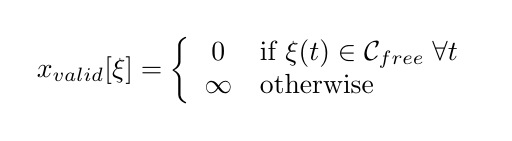
\begin{tikzpicture}
      \node at (0,0) {
         $\arraycolsep=5pt%
         x_{\ms{valid}}[\xi] = \left\{ \begin{array}{cl}
            0 & \mbox{if } \xi(t) \in \mathcal{C}_{\ms{free}} \;\forall t \\
            \infty & \mbox{otherwise} \\
         \end{array} \right.$
      };
   \end{tikzpicture}
   \caption{Edge cost model
      for the (feasible) motion planning problem.}
   \label{fig:roadmaps:cost-model-feasible}
\end{marginfigure}

\paragraph{The Motion Planning Problem.}
Consider a single-pair motion planning query $u$
consisting of start and destination vertices
$q_{\ms{start}}, q_{\ms{dest}} \in \mathcal{C}$
as well as a collision-free subset $\mathcal{C}_{\ms{free}}$.
The motion planning problem consists of finding a valid path $\xi^*$
with $\xi^*(0) = q_{\ms{start}}$ and $\xi^*(1) = q_{\ms{dest}}$
if one exists.

\subsection{Optimal Motion Planning}

\begin{marginfigure}
   \centering
   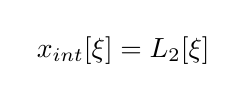
\begin{tikzpicture}
      \node at (0,0) {
         $x_{\ms{int}}[\xi] = L_2[\xi]$
      };
   \end{tikzpicture}
   \caption{Example dynamical cost function for the optimal
      motion planning problem.
      Here, the arc length of $\xi$ using the $L_2$ norm cost is used.}
   \label{fig:roadmaps:cost-model-path}
\end{marginfigure}

The \emph{optimal motion planning problem}
is a generalization of the motion planning problem which
includes an additional objective over solution paths
$x_{\ms{int}} : \Xi \rightarrow \mathbb{R}$
intended to measure properties intrinsic to the path.
Common choices for $x_{\ms{int}}$ include
the path's arc length,
the total time or energy necessary to execute the path,
or the squared time derivatives averaged over the path.
See \citep{karaman2011samplingoptimal} for a comprehensive treatment
of sampling-based methods for the optimal motion planning problem.

\marginnote{An optimal motion planner
   typically considers both feasibility dynamical properties of candidate paths --
   this objective is simply $x_{\ms{opt}} = x_{\ms{valid}} + x_{\ms{int}}$.
   We treat them separately because they exhibit fundamentally different
   computational profiles.}

\subsection{Further Generalizations}

There are a great number of further generalizations of the
motion planning problem that we will not explicitly consider.
For example,
the kinodynamic planning problem includes the derivatives of the
configuration variables,
and a solution to the kinodynamic problem is called a trajectory.
%Various algorithms exist \citep{lavallekuffner1999rrt}.
The objective used in optimal variants of the kinodynamic problem
often include terms which depend on the accelerations or control
inputs (e.g. torques)
required to execute the trajectory.

Constrained motion planning constitutes a different generalization.
A holonomic constraint on the configuration space,
for example,
induces a subset (often a manifold) of the configuration space
on which planning is restricted.
Various motion planners \citep{berenson2009manifolds}
have been proposed to accommodate such constraints.

\section{Motion Planning by Discretizing C-Space}

While the generalized mover's problem is computationally hard
\citep{reif1979moverscomplexity},
a large array of algorithms have been proposed that perform
well on a large range of typical instances.
We give a brief review of approaches to the motion planning problem
that rely principally on discretizations of the configuration space.

\subsection{Building Graphs in C-Space}
\label{subsec:roadmaps:building-graphs}

\paragraph{Testing Validity of Configurations.}
How can we establish the validity of a configuration $q$?
This question is especially delicate when the geometry is complex
and the configuration-space obstacles cannot be represented explicitly.
In this case,
it is necessary to test prospective paths
for membership in $\mathcal{C}_{\ms{free}}$ using a predicate
that we express as a binary-valued
\emph{indicator function},
\begin{equation}
   \mathbf{1}_{\mathcal{C}\ms{free}} : \mathcal{C} \rightarrow
      \{ \mbox{True}, \mbox{False} \} 
   \mbox{\quad s.t. \quad}
   \mathbf{1}_{\mathcal{C}\ms{free}}(q) = \mbox{True} \mbox{ iff } q \in \mathcal{C}_{\ms{free}}.
\end{equation}
Note that implementing $\mathbf{1}_{\mathcal{C}\ms{free}}$ for an articulated robot
entails computing the forward kinematics of the robot at the
query configuration,
and conducting a collision check in the workspace.

\paragraph{Testing Validity of Paths.}
How can we establish the validity of a path $\xi$
according to (\ref{eqn:roadmaps:path-validity})?
There are many approaches that can be applied,
including C-space bubbles \citep{quinlan1994modification}
and computing a path discretization resolution and corresponding
workspace obstacle padding
\citep{barraquand1991distributedrepresentation}.
We will generally assume that a functional variant of the indicator
function is available:%
\marginnote{The experiments in this document commit to a particular
collision checking resolution for motion validity.}%
\begin{equation}
   \mathbf{1}_{\Xi\ms{free}} : \Xi \rightarrow
      \{ \mbox{True}, \mbox{False} \} .
\end{equation}

\paragraph{Motion Planning as Pathfinding.}
Importantly,
two paths $\xi_{ab}$ and $\xi_{bc}$ with $\xi_{ab}(1) = \xi_{bc}(0)$
can be concatenated to a path $\xi_{ac}$,
with
\begin{equation}
   \mathbf{1}_{\Xi\ms{free}}(\xi_{ab})
   \;\land\;
   \mathbf{1}_{\Xi\ms{free}}(\xi_{bc})
   \iff
   \mathbf{1}_{\Xi\ms{free}}(\xi_{ac}).
\end{equation}
This motivates approaches which maintain a graph structure of
smaller valid motions in the configuration space.
Consider a graph $G = (V,E)$,
with each vertex $v \in V$ a configuration $q_v \in \mathcal{C}$,
and each edge $e_{uv} \in E$ a path $\xi_e \in \Xi$
s.t. $\xi(0) = q_u$ and $\xi(1) = q_v$,
and consider vertices $v_{\ms{start}}, v_{\ms{dest}} \in V$
corresponding to query vertices $q_{\ms{start}}, q_{\ms{dest}}$.
Then a path $p$ through $G$ from
$v_{\ms{start}}$ to $v_{\ms{dest}}$,
on which each edge $e$ has $\mathbf{1}_{\Xi\ms{free}}(\xi_e) = \mbox{True}$,
corresponds to a valid solution to the motion planning problem.

\paragraph{Optimal Motion Planning as Pathfinding.}
Furthermore,
if the intrinsic optimization objective $x_{\ms{int}}$
from Figure~\ref{fig:roadmaps:cost-model-path} is \emph{additive},
then the optimal motion planning problem can be solved on $G$
via a shortest path algorithm
(at least up to the discretization afforded by the graph).
This is accomplished by defining an edge weight function
$w : E \rightarrow \mathbb{R}$
by $w(e) = x_{\ms{opt}}(\xi_e)$.

A wide variety of approaches exist in the literature for
constructing, searching, and validating this graph
for motion planning problems.
We will broadly review a selection of different algorithms later
in this chapter (Section~\ref{sec:roadmaps:sensitivity}).

%\paragraph{Resolution and Probabilistic Completeness.}
%Any discretization is only an approximation of the actual configuration
%space.
%Of course, the discretization is always just an approximation
%of the actual C-space.
%Hopefully, you can choose a discretization strategy that allows your
%algorithm to have one or both of these forms of completeness.

%\paragraph{Motion Planning as Pathfinding.}
%\label{subsec:roadmaps:planning-as-pathfinding}
%Here, talk about how even if there are multiple available
%start or goal configurations
%(e.g. different grasps or inverse kinematics solutions),
%the motion planning problem can still be posed as a
%single-pair shortest path (SPSP) problem
%by augmenting the graph with virtual source sink vertices
%and edges.

\paragraph{Other Approaches to Motion Planning.}
The motion planning problem affords a number of different classes of
algorithms,
many of which do not construct graphs of local motions in the
problem's configuration space.
Potential field methods \citep{khatib1986potentialfields}
and navigation functions \citep{rimon1989navigationfunctions}
construct fields whose gradients can guide a path around
local obstacles.
Trajectory optimization approaches are especially well-suited to
planning instances in which the basins of attraction are large.
Approaches such as CHOMP \citep{zucker2013chomp}
and TrajOpt \citep{schulman2013trajopt})
commit to a trajectory representation for $\xi^{(1)}$
and use require stronger world descriptions
(SDFs, convex obstacle decompositions)
to make local modifications
to produce a new path $\xi^{(2)}$.
Also,
optimizers are commonly used in lower levels to react to local
changes (e.g. \citep{quinlan1994modification}).

\section{Obstacle Sensitivity}
\label{sec:roadmaps:sensitivity}

Generally,
graph-based motion approaches as described
in Section~\ref{subsec:roadmaps:building-graphs}
require the following three processes:
(a) constructing the graph,
(b) searching the graph, and
(c) validating the graph.
One of the key differentiators between the many graph-building
techniques for motion planning
is how they interleave these three processes.
This section considers one important factor:
the degree of dependence of the graph structure
on the distribution of obstacles in the scene.
We broadly categorize algorithms into two groups:
those that are \emph{obstacle-sensitive},
and those that are \emph{obstacle-insensitive}.

\subsection{Obstacle-Sensitive Approaches}
\label{subsec:roadmaps:sensitive}

In an obstacle sensitive approach,
the graph is built incrementally,
and construction of new elements (e.g. vertices and edges)
is directly interleaved with validating those elements
in response to the distribution of valid or costly states.
These approaches might be best understood
as constructing an approximation to $\mathcal{C}_{\ms{free}}$
as directly as possible.

\paragraph{Exact Algorithms.}
The earliest work on the motion planning problem studied
\emph{exact} or \emph{semi-algebraic}
algorithms which worked directly on an explicit representation
of the obstacles (e.g. polygons) in the configuration space
\citep{lozanoperez1983cspace}.
This formulation of motion planning was shown to be
PSPACE-hard \citep{reif1979moverscomplexity,canny1988complexitymotionplanning}.
These approaches can guarantee optimal solutions,
and may be even be able to guarantee the validity of certain edges
by construction.
However,
they are difficult to apply to problems on articulated
robots for two reasons.
First, many approaches are only applicable to problems
in two or three dimensions,
or to robots with only translational degrees of freedom
\citep{kavraki1995cspacefft}.
Second, an explicit representation of obstacles in the
configuration space is exceedingly difficult to achieve due to the
nonlinearity in the forward kinematics function.
While some approaches are able to construct explicit
analytical or approximate configuration space obstacles from
workspace geometry (e.g. \citep{newmanbranicky1991cspacetransforms}),
they are often only applicable to simple kinematics.

\paragraph{Treebuilding Algorithms.}
Many approaches do treat the configuration space implicitly
(i.e. using indicator functions for validity checking as described
in Section~\ref{subsec:roadmaps:building-graphs}).
The most common algorithms simultaneously grow and validate trees,
either unidirectionally from the $v_{\ms{start}}$ or bidirectionally
from both start and goal configurations.
At each iteration,
these algorithms use a sampling strategy to propose a new extension,
and then augment their tree(s) if the new motion is found to be valid.
Key examples of this approach include
Expansive Space Trees (EST) \citep{hsu1997expansive}
and Rapidly-exploring Random Trees (RRT)
\citep{lavalle1998rrt, kuffner2000rrtconnect}.
The SBL planner \citep{sanchezante2001sbl}
is a bidirectional variant of EST with lazy edge validity checking.

\paragraph{Planning vs. Execution Cost.}
The foundational algorithms in this category are primarily concerned
with path \emph{feasibility} -- that is, the objective $x_{\ms{valid}}$
from Figure~\ref{fig:roadmaps:cost-model-feasible};
there is often no mechanism explicitly biasing them to select
low-cost paths.
\marginnote{We talk about this tradeoff between planning and
execution cost in detail in Chapter~\ref{chap:utility}.}
Therefore, solutions found tend to be of low quality,
and they are customarily optimized using a path shortcutting
algorithm in a post-processing phase before they can be executed.
More recent work has also focused on asymptotically optimal variants
of these planners
\citep{karaman2010rrtstar, karaman2011samplingoptimal, gammell2015bitstar, hauser2015lazy}
which do address more general cost objectives.

\paragraph{Advantages of Obstacle Sensitivity.}
One key advantage to obstacle-sensitive approaches is that
they only construct the graph structure in the parts of the
configuration space that are relevant to the planning query.
The Voronoi sampling bias of the RRT or the importance sampling of the EST
attempt to focus graph construction in areas of the configuration space
which tend to find feasible paths quickly.
These techniques can also take account of the current distribution
and connectivity of the discretization in order to focus new
samples to their advantage
(e.g. to address the narrow passage problem),
such as visibility tests \citep{simeon2000visibilityprms}
or the expansion phase of the original PRM
\citep{kavrakietal1996prm}.
These heuristics can also be incorporated into sampling-based planners
as obstacle-based \citep{boor1999prmgaussiansampling}
or hybrid \citep{hsu2005hybridsampling} sampling strategies.

An additional advantage of these approaches
is that they handle densification naturally.
The graph structure is augmented automatically,
so the resolution of the discretization need not be explicitly
increased as the instance reveals itself to be more difficult.

%Probabilistic completeness.

\subsection{Obstacle-Insensitive Approaches}

In contrast to obstacle-sensitive approaches,
the approaches we describe here
commit to a particular discretization
of the configuration space a priori,
independent of the distribution of obstacles.
While this simpler method forgoes some of the advantages of
obstacle sensitivity discussed previously,
this independence does confer some advantages of its own.

\paragraph{Roadmap Methods.}

The foundational obstacle-insensitive methods particular to the motion
planning problem are called \emph{roadmap methods}.
The term roadmap usually connotes a graph embedded in a continuous
ambient space in the presence of obstacles.
Vertices in the graph,
which correspond to configurations in the configuration space,
are also called milestones.
The first roadmap methods such as the
Probabilistic RoadMap (PRM) \citep{kavrakietal1996prm}
initialized the milestones arrangement
from a uniform distribution over the free space.

Key to roadmap methods to motion planning
is the concept of the \emph{local planner}
which governs the validity of roadmap edges.
Given two configurations $q_a, q_b \in \mathcal{C}$,
the local planner considers a candidate path $\xi_{ab}$ between
them.
(A common implementation simply uses the straight-line path
in configuration space.)
Edges are only attempted when they meet certain restrictions,
such as distance with respect to some metric.

There are some variants of roadmap planners that are not independent
of the obstacle distribution.
First,
many roadmap planners make use of a heuristic ``expansion'' step
wherein additional samples are added to the roadmap
in order to increase its connectivity.
Second,
edge connection rules that can forgo connections within
the same connected component.

%\cdnote{Densification?}

\paragraph{Search-based Methods.}
Graph pathfinding algorithms such as A* \citep{hart1968astar}
are applicable to the motion planning problem if a suitable
discretization of the continuous space is considered.
While roadmaps can serve as this discretization,
application of search-based methods often represents the space
implicitly via a set of operators or motion primitives
which reproduce a regular lattice over the configuration space
\citep{pivtoraiko2005statelattice}.
When the vertices comprising the lattice are rectangular
(also called a Sukharev point set \citep{sukharev1971extremum}),
search-based planning is also called ``grid search.''
Such search methods can exploit a vertex heurstic,
and many heuristics have been proposed for articulated motion planning
-- the most common of which compute a decomposition over the
lower-dimensional workspace to guide the search.
Some methods \citep{plaku2010syclop} exploit synergies between these
different levels of planning to achieve more efficient planning.

\paragraph{Lazy Validity Checking.}
Because obstacle-insensitive approaches decouple graph construction
from validity checking,
it is often advantageous to defer the latter until it is
necessary for solving the query at hand.
Lazy validity checking has been exploited
in roadmap methods such as the Lazy PRM
\citep{bohlin2000lazyprm, hauser2015lazy},
search methods such as Lazy Weighted A* \citep{cohen2014narms},
and methods which bridge the two
such as Fast Marching Trees (FMT*) \citep{janson2015fmtstar}
and Bidirectional FMT* (BFMT*) \citep{starek2015bfmtstar}.
We discuss laziness in the context of graph search
more comprehensively in Chapter~\ref{chap:lazysp}

\paragraph{Adaptive Densification.}
One difficulty with these obstacle-insensitive approaches
is that they commit to a particular discretization,
and once their search is exhausted,
they must return the best path found,
or report failure if no path was found.
This property is known as resolution completeness
\citep{cheng2004rescomplete}.

Many instance of prior work endeavor to progressively
densify their discretization until a suitable solution is found.
Early examples of this approach include
hierarchical cell decompositions \citep{faverjon1984octree}
and workspace and C-space bitmap pyramids for search over potential fields
\citep{barraquand1991distributedrepresentation}.
More recent asymptotically optimal motion planners such as
Lazy PRM* \citep{hauser2015lazy}.
and BIT* \citep{gammell2015bitstar} take a similar approach to
roadmap search,
which we also adopt as described in Chapter~\ref{chap:utility}
(see Figure~\ref{fig:roadmaps:roadmap-stack}).

\begin{figure}
   \centering
   \includegraphics{build/roadmap-stack}
   \caption{A stack of progressively densified roadmaps
      over a given configuration space $\mathcal{C}$.
      Each deeper roadmap constitutes a more accurate approximation
      to the true continuous problem space.}
   \label{fig:roadmaps:roadmap-stack}
\end{figure}

\paragraph{Advantages of Obstacle Insensitivity.}
The obstacle sensitivity question represents an underlying efficiency
tradeoff.
Sensitive approaches may be able to adapt their discretization more
directly to local obstacle distributions.
On the other hand,
insensitivity to obstacles admits a number of efficiency advantages.
Much of the nearest-neighbor computation
often required during graph construction can be cached and amortized
over all planning queries.
Other properties of the discretization that are constant between
similar planning instances can also be shared
as described in Chapter~\ref{chap:family}.
For these reasons,
this thesis build on top of obstacle-insensitive roadmaps.

\section{Roadmap Classes}
\label{sec:roadmaps:roadmap-classes}

Roadmap methods operate over a graph constructed in the
robot's configuration space.
Roadmap milestones are commonly generated by a number of different
types of point sequences,
and edges are considered between vertices pairs that meet
certain constraints.
While most algorithms methods are generally agnostic
to the class of roadmap that they operate on,
choosing a suitable class and its parameters has a large effect
on both theoretical and practical performance.

\paragraph{Random Sequences.}
The original roadmap algorithms
\citep{kavrakietal1996prm}
operated primarily over sets
of vertices drawn uniformly at random from the configuration space.
Many more recent algorithms such as
RRT* \citep{karaman2010rrtstar},
PRM* \citep{karaman2011samplingoptimal},
FMT* \citep{janson2015fmtstar},
RRT$^{\#}$ \citep{arslan2013rrtsharp},
and BIT* \citep{gammell2015bitstar} make use of the same
uniform obstacle distribution.
Such a distribution is attractive both because
it is simple to implement
it because it allows for theoretical properties such as
completeness and optimality to be demonstrated
in probability.

\paragraph{Deterministic Sequences.}
Many researchers have examined whether randomness is a necessary
(or even beneficial) aspect of treebuilding and roadmap planners
\citep{branicky2002detvsprobroadmaps}.
This is especially relevant in the context of comparing
roadmap planners with search-based methods
that conventionally operate over lattices \citep{lavalle2002gridprms}.

One of the most straightforward disadvantages of using a
non-deterministic sequence for each motion planning query
is that the constructed graph is different for each query.
This makes it impractical to pre-compute and amortize nearest
neighbor queries across problem instances,
as well as to pre-compute edge states as described in
Chapter~\ref{chap:family}.

Further,
theoretical properties of roadmap methods
such as resolution completeness and asymptotic optimality
depend on properties of the underlying point set
such as its \emph{dispersion}.
Not only can the dispersion of a set of randomly sampled points
only be established in expectation,
but it is demonstrably larger than the dispersion of other
well-known point sequences,
such as the Halton or Hammersley set,
or the Sukharev grid.
For an in-depth analysis of different point sets for roadmap
planning, see Janson \citep{janson2015deterministicsampling}.

\begin{figure}
   \centering
   \includegraphics{build/roadmaps/gen/aagrid}
   \;
   \includegraphics{build/roadmaps/gen/rgg}
   \;
   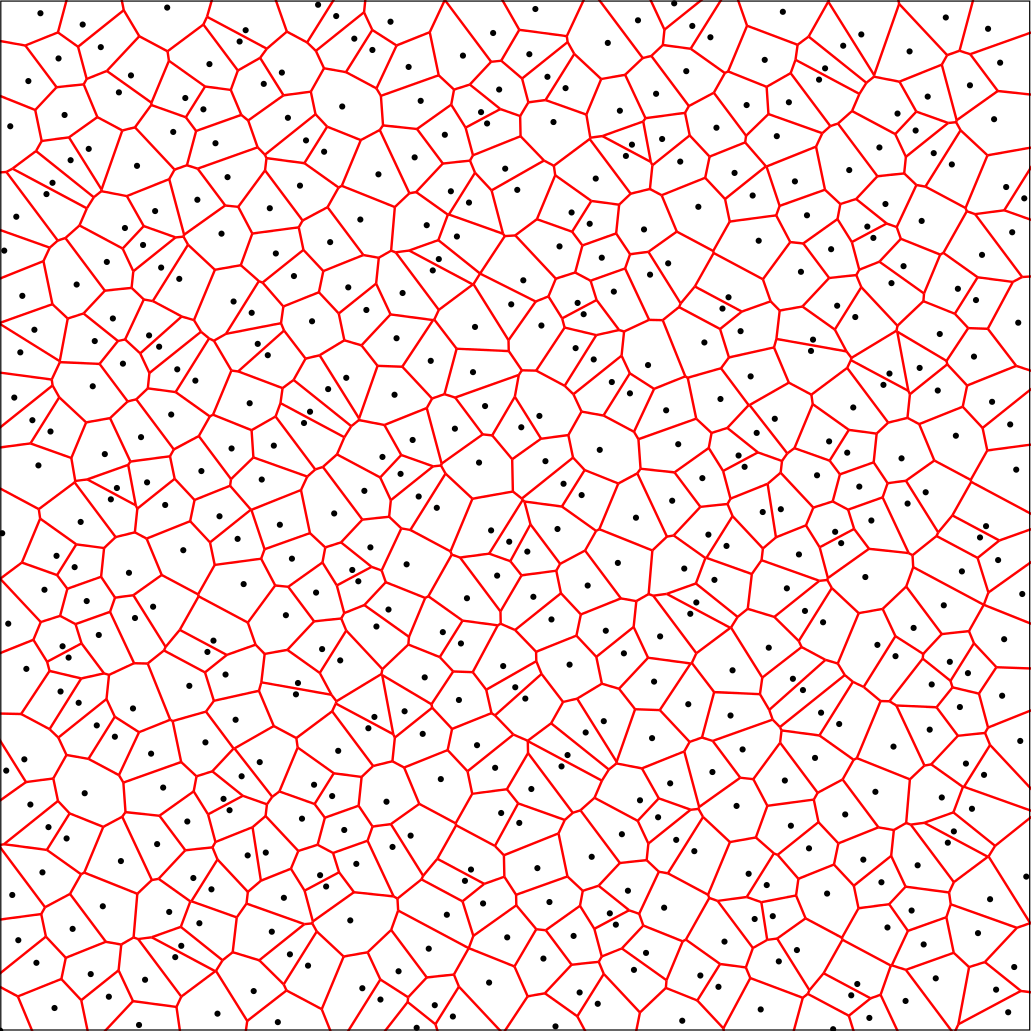
\includegraphics{build/roadmaps/gen/halton}
   \caption{Examples of three roadmap types over the unit square:
      an axis-aligned lattice (left),
      random geometric graph (middle),
      and Halton graph with primes $(2,3)$ (right).
      All three roadmaps have a connection radius of 0.3.
      The latter two roadmaps have 30 vertices.}
\end{figure}

\paragraph{Connection Radii.}
Previous work \citep{karaman2011samplingoptimal} has established
that a roadmap planner which uses a uniformly randomly generated
point set is asymptotically optimal almost surely
if the edge connection radius $r$ is sufficiently large w.r.t.
the number the number of samples $n$.
In particular,
it defines the critical value $\gamma^*_{\mathcal{C}}$:
\begin{equation}
   \gamma^*_{\mathcal{C}}
      = 2 \left( \left[ 1 + \frac{1}{d} \right]
         \frac{\lambda_d(\mathcal{C})}{\zeta_d} \right)^{1/d},
\end{equation}
where $d$ is the dimensionality of the configuration space,
$\lambda_d(\cdot)$ represents the Lebesgue measure (e.g. volume),
and $\zeta_d$ is the Lebesgue measure of the $d$-dimensional unit ball.
Note that while other publications consider $n$ to be the number
of milestones in the collision-free subset of the space
(and therefore also rely on the measure of that subset),
we measure the volume of the entire C-space,
and let $n$ correspond to the total number of vertices.
We do this because we will be determining the validity of roadmap edges
in a separate step,
as described in Chapter~\ref{chap:lazysp}.

Asymptotic optimality under uniform sampling requires
an edge connection radius $r_{\ms{log}}$:
\begin{equation}
   r_{\ms{log}}(n) =  \gamma^*_{\mathcal{C}} \, \eta
      \left( \frac{\log(n)}{n} \right)^{1/d}
\end{equation}
for some tuning parameter $\eta > 1$.
Point sets with tighter dispersion bounds,
such as the Halton sequence,
can exploit a smaller connection radius $r_{\ms{loglog}}$:
\begin{equation}
   r_{\ms{loglog}}(n) = \gamma_{\mathcal{C}} \, \eta
      \left( \frac{\log(\log(n))}{n} \right)^{1/d}.
\end{equation}
For details we refer the reader
to \citep{janson2015deterministicsampling}.

\begin{margintable}
   \centering
   {\renewcommand{\tabcolsep}{0.15cm}
   \begin{tabular}{lccc}
      \toprule
      & HERB & CHIMP & IRB 4400 \\
      \midrule
      $d$ & 7 & 7 & 6 \\
      $\gamma^*_{\mathcal{C}}$ & 7.67 & 7.97 & 7.74 \\
      $r_{\ms{log}}$ & 2.83 & 2.93 & 2.41 \\
      $r_{\ms{loglog}}$ & 2.31 & 2.40 & 1.90 \\
      \bottomrule
   \end{tabular}
   }
   \vspace{0.1cm}
   \caption{Table of roadmap connection radii parameters for
      various scaling rates across the different robot platforms
      considered in this thesis.
      Radii presented are for $n=10000$ and $\eta = 1$,
      and are given in radians.}
   \label{table:roadmap-params}
\end{margintable}

\paragraph{Roadmaps for Articulated Robots.}
We apply roadmap methods to the three robot platforms
from Chapter~\ref{chap:intro} in this thesis.
Unless otherwise noted,
we build roadmaps directly in the joint space of the robot.
See Table~\ref{table:roadmap-params} for the roadmap parameters
that we use.

%\cdnote{Add a plot of roadmap sizes for each batch
%for each robotic platform}.

%\subsection{Dispersion}
%
%Deterministic sampling and dispersion:
%\citep{janson2015deterministicsampling}.
%
%\begin{figure}
%   \centering
%   \includegraphics{build/roadmaps-dispersion/dispersion}
%   \caption{Dispersion plot on the unit square.
%      Green is the dispersion of an incremental (greedy) Sukharev
%      grid.}
%\end{figure}
%
%\begin{figure}
%   \centering
%   \includegraphics{build/roadmaps-dispersion/dispersion-herb}
%   \caption{HERB dispersion plot.}
%\end{figure}
%
%\begin{figure}
%   \centering
%   \includegraphics{build/roadmaps-dispersion/dispersion-irb4400}
%   \caption{IRB4400 dispersion plot.}
%\end{figure}

%\subsection{Batch Size}
%
%\begin{figure}
%   \centering
%   \begin{tikzpicture}
%   \begin{axis}[
%         xmode=log,
%         xlabel={Batch Size},
%         ylabel={LazySP Time (s)},
%         xlabel near ticks,
%         ylabel near ticks,
%         ]
%      \addplot coordinates {
%         (100, 0.2407595708)
%         (250, 0.27367886569999994)
%         (1000, 0.2165730066)
%         (2500, 0.3836524094)
%         (10000, 0.47772694290000006)
%      };
%   \end{axis}
%   \end{tikzpicture}
%   \caption{Batch size. {\tt herbbin0}, seeds 1-10, gammafac=1, lambda=0.}
%\end{figure}
